\documentclass{standalone}
\usepackage{tikz}

\begin{document}
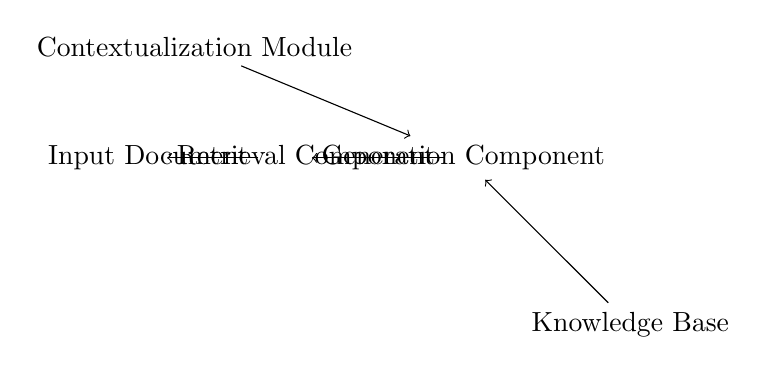
\begin{tikzpicture}[node distance=2cm, auto]
  % Nodes
  \node (input) {Input Document};
  \node [right of=input] (retrieval) {Retrieval Component};
  \node [right of=retrieval] (generation) {Generation Component};
  \node [below right of=generation, node distance=3cm] (kb) {Knowledge Base};
  \node [above left of=retrieval, node distance=2cm] (contextualization) {Contextualization Module};

  % Edges
  \draw[->] (input) -- (retrieval);
  \draw[->] (retrieval) -- (generation);
  \draw[->] (kb) -- (generation);
  \draw[->] (contextualization) -- (generation);
\end{tikzpicture}
\end{document}